\documentclass[a4paper,12pt]{report}
\usepackage[francais]{babel}
\usepackage[T1]{fontenc}
\usepackage[utf8]{inputenc}
\usepackage{titlesec}
\usepackage{minted}
\usepackage{graphicx}

\usepackage[top=3.0cm]{geometry}
\usepackage{color}
\definecolor{grey}{rgb}{0.99,0.99,0.99}
\titleformat{\chapter}[hang]{\bf\huge}{\thechapter}{2pc}{}

\setcounter{secnumdepth}{3}
\setcounter{tocdepth}{3}
        
\begin{document}

\begin{titlepage}
\begin{center}
\end{center}

\flushright
\begin{center}
\bigskip
\bigskip
\bigskip
\bigskip
\bigskip
\bigskip
\bigskip
\bigskip
\bigskip
\bigskip
\bigskip
\bigskip
\huge{Projet de langage object avancé : Gestionnaire de contacts}\\
\end{center}
\begin{center}
\bigskip
\bigskip
\bigskip
\bigskip
\bigskip
\bigskip
\bigskip
\bigskip
\bigskip
Romain Beaumont et Thomas Lourseyre\\
\bigskip
\bigskip
\bigskip
\bigskip
\bigskip
\bigskip
\bigskip
\bigskip
\bigskip
\bigskip
\bigskip
\bigskip
\bigskip
\bigskip
\bigskip

\textbf{du} 12 Mars 2013  \textbf{au} 2 Avril 2013

\bigskip
\bigskip
\bigskip
\end{center}
\end{titlepage}
 
\tableofcontents


\chapter{Introduction}
\par
L'objectif de ce projet est de réaliser un gestionnaire de contact en utilisant Qt et la stl.

\section{Spécifications}

Voici les différentes spécifications qui ont été données :
\begin{itemize}
	\item Concevoir des classes permettant d'implémenter une liste de contacts et les champs qui permettront de les caractériser
	\item Concevoir une interface graphique en utilisant Qt
	\item Implémenter l'import/export des données de l'application sous deux formats : le format vCard et un format personnalisé
	\item Concevoir la documentation du projet en utilisant Doxygen.\\
\end{itemize}

Le projet se divise en trois parties :
\begin{itemize}
	\item La conception du modèle : trouver une hiérarchie pratique et efficace
	\item Implémentation des fonctionnalités : rendre le projet fonctionnel
	\item La conception de l'interface graphique : donner à l'utilisateur accès à toutes les fonctionnalités
\end{itemize}


\section{Fichiers et dossiers du projet}

\begin{itemize}
	\item \texttt{ProjetLOA.pro} est le fichier de description du projet (our \texttt{qtcreator})
	\item \texttt{main.cpp} contient la fonction \texttt{main} du projet
	\item \texttt{controleur/}, \texttt{modele/} et \texttt{vue/} sont les dossiers où sont mises les sources
	\item \texttt{html/} et \texttt{latex/} sont les dossier où sont enregistré la documentation
	\item \texttt{rapport/} est le dossier où se trouve ce rapport
	\item \texttt{icone/} et \texttt{dia/} sont les dossiers regroupant icones et diagramme
	\item \texttt{ressources.qrc} est le fichier ressource du projet
	\item \texttt{loadoc} est le fichier de configuration de \texttt{doxygen}
\end{itemize}

\chapter{Hiérarchie des classes}
\par
Voici un diagramme de classe résumant les héritage et aggrégats :
\par
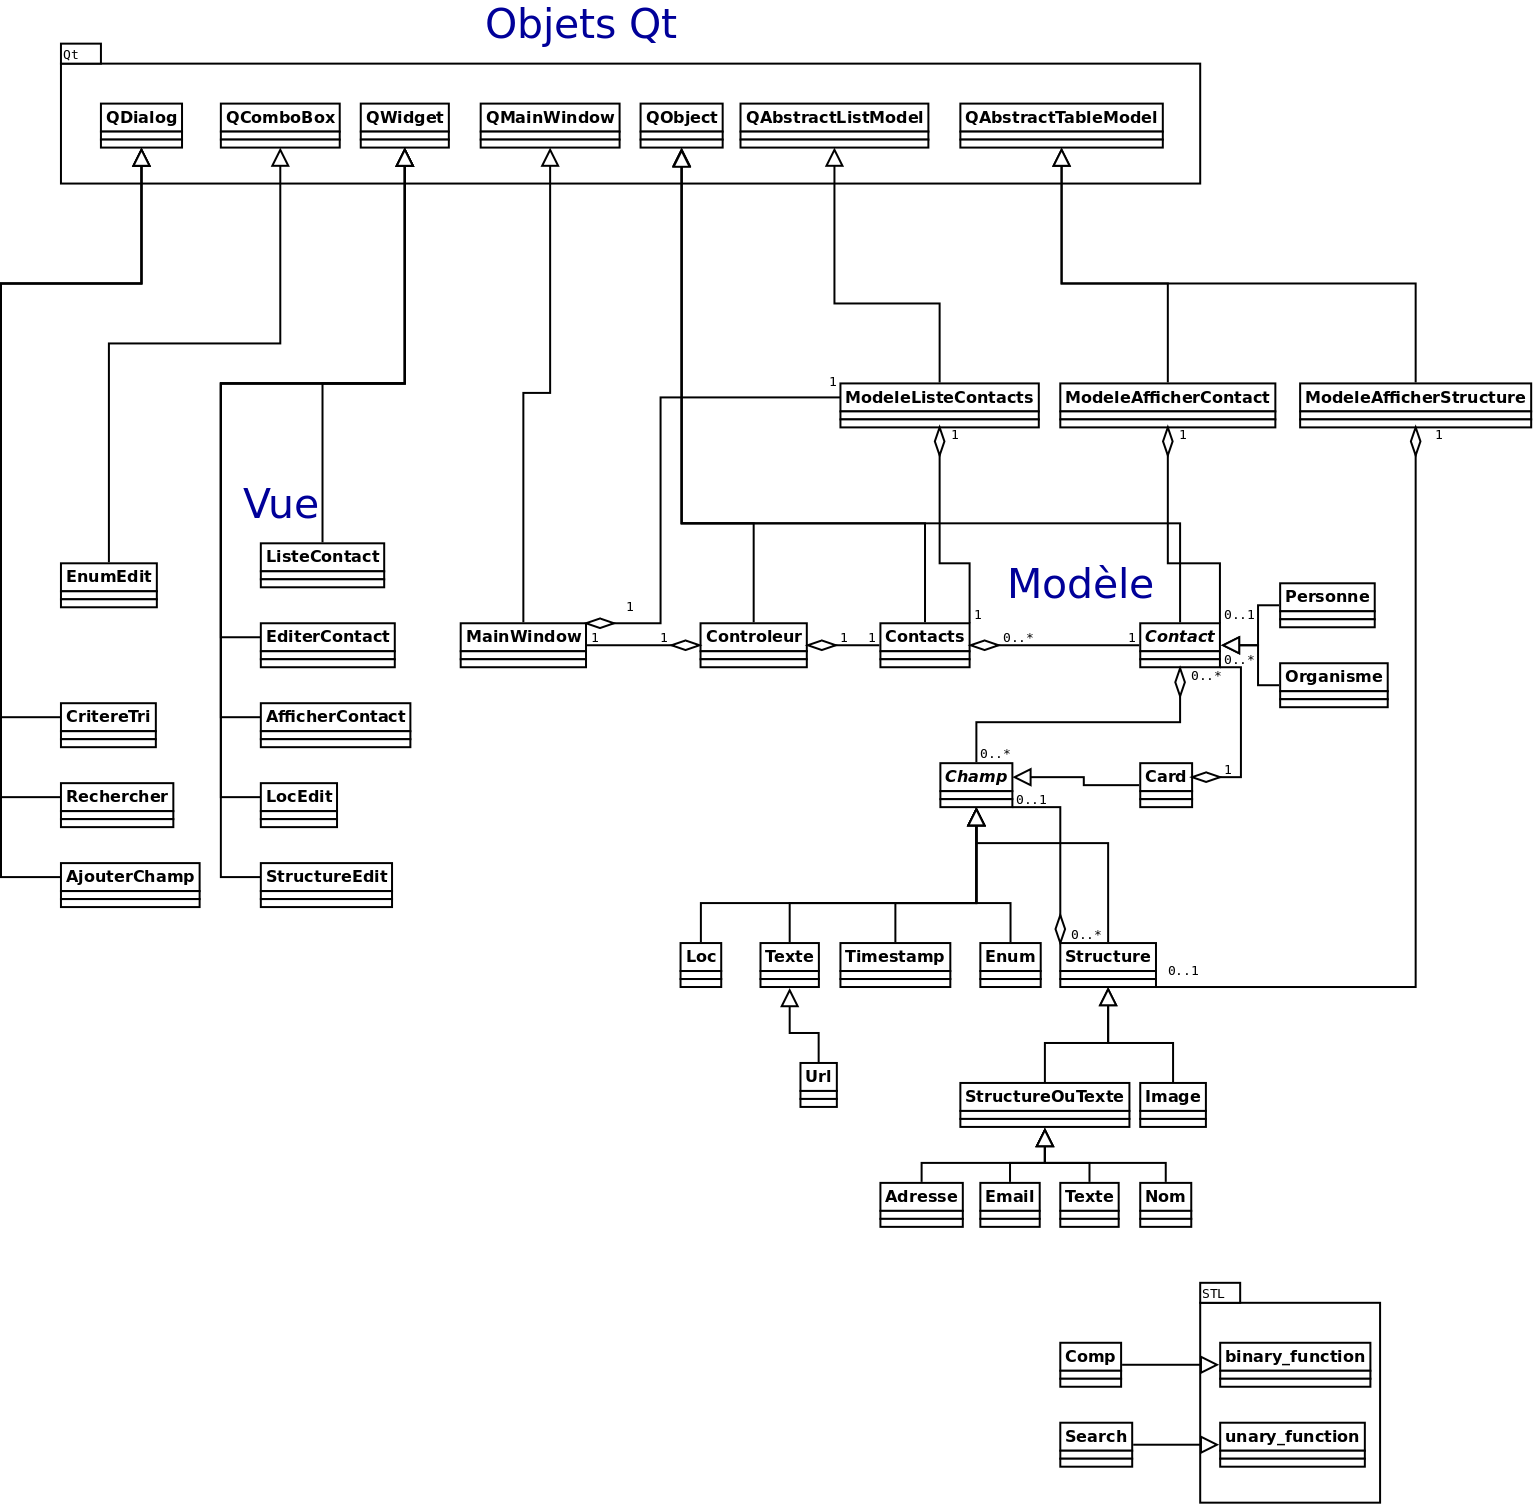
\includegraphics[scale=0.2]{../dia/ClassDiagram.png}
\par
La documentation du projet est disponible au format HTML (\texttt{./html/index.html}) et au format pdf (\texttt{./latex/refman.pdf}).
Elle a été générée en utilisant \texttt{doxygen}.

\section{Contrôleur}

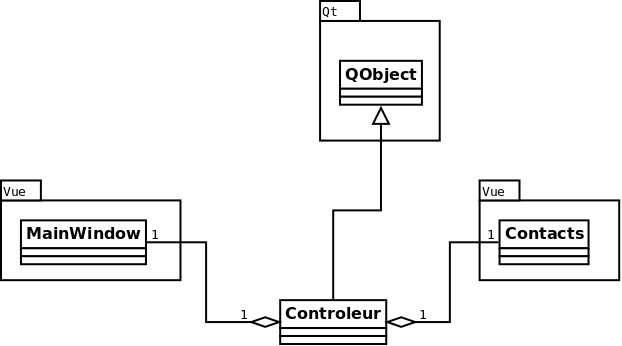
\includegraphics[scale=0.35]{../dia/ClassDiagramControler.png}

La partie controleur de l'application s'occupe uniquement de lier les signaux et les slots des classes de la vue et du modèle entre elles.

L'unique classe du contrôleur instancie un objet \texttt{MainWindow} (de la partie vue) et un objet \texttt{Contacts} (de la partie modèle), et les connecte entre eux.

\section{Modèle}

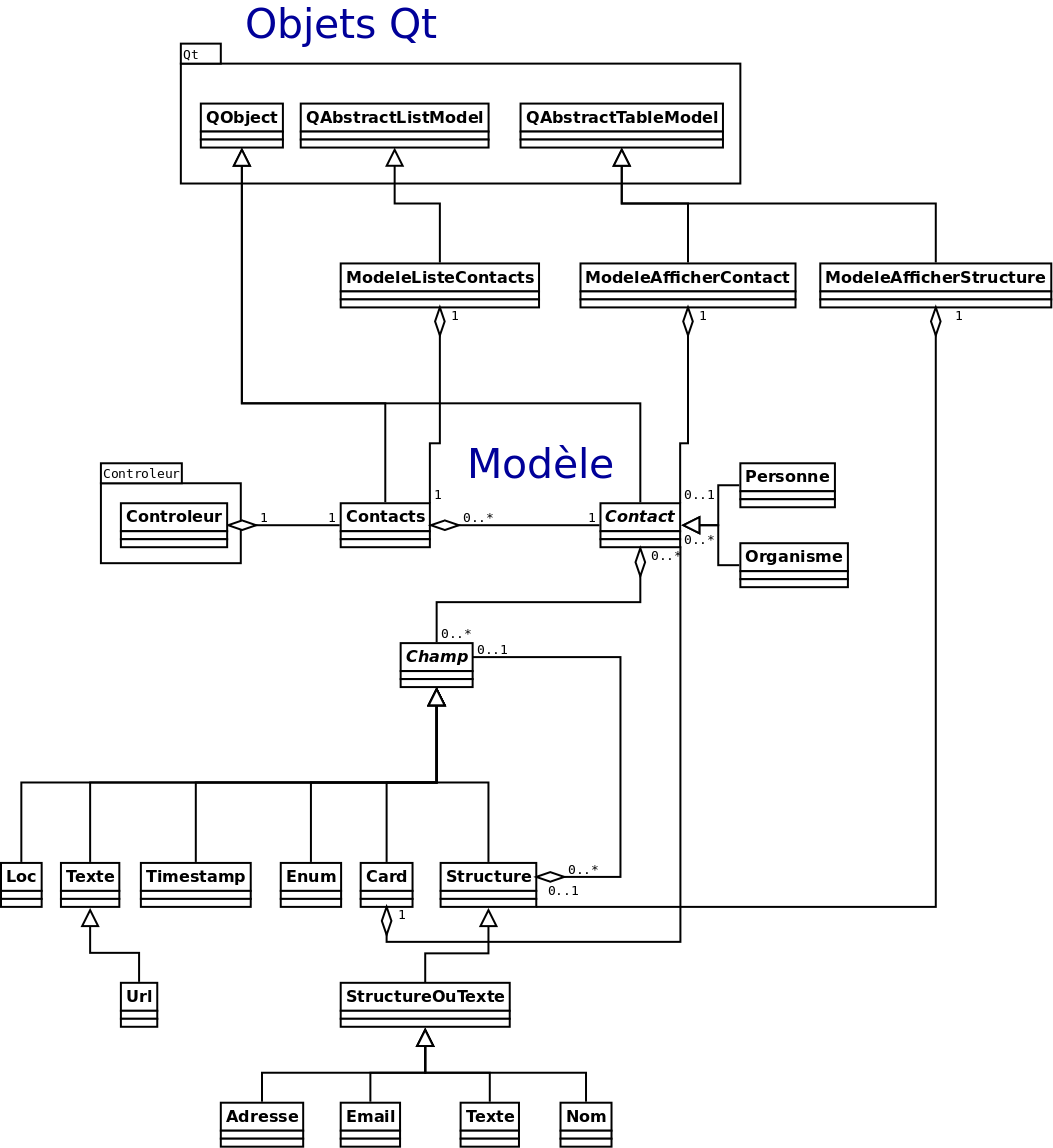
\includegraphics[scale=0.3]{../dia/ClassDiagramModel.png}

Le modèle consiste en une classe \texttt{Contact\bf{s}} tout en heut de la hiérarchie, qui implémente une liste de \texttt{Contact}.
Cette dernière est abstraite car d'elle hérite deux templates de \texttt{Contact}, \texttt{Personne} et \texttt{Organisme}, qui ne font que définir les valeurs de champ possibles et par défaut.

\texttt{Contact} contient une liste de \texttt{Champ}, qui est une classe abstraite car d'elle hérite toutes les implémentations de champ géré par l'application.
La plupart des filles de \texttt{Champ} utilise leur propre implémentations, hormis \texttt{Card} qui instancie un Contact (représentant soit une personne, soit un organisme) et \texttt{Structure}, qui implémente un champ avec plusieurs entrées, instanciant donc une liste de \texttt{Champ}. Elle possède deux filles correspondant à des structures particulières : \texttt{Image} et \texttt{StructureOuTexte} qui elle-même possède quatre filles : \texttt{Adresse}, \texttt{Email}, \texttt{Text} et \texttt{Nom}.

Les classes \texttt{ModeleListeContact}, \texttt{ModeleAfficherContact} et \texttt{ModeleAfficherStructure} sont des modèles Qt qui permettent à la vue de gérer correctement l'affichage (qui permet de modifier dynamiquement l'affichage).

Il y a également deux foncteurs : \texttt{Comp} et \texttt{Search}. Elles sont aggréguées dans plusieurs classes qui n'ont pas été mentionnées sur le diagramme par soucis de lisibilité.
\texttt{Comp} est l'opérateur binaire de comparaison entre les \texttt{Contact}. Elle prend en entrée deux {\bf pointeurs} de \texttt{Contact}, compare les contacts pointés selon le critère passé en argument dans le constructeur et renvoie un booléen.
\texttt{Search} est un opérateur unaire qui cherche le contact dont le nom est donné dans le constructeur dans l'objet \texttt{Contact*} passé à l'opérateur.


\section{Vue}

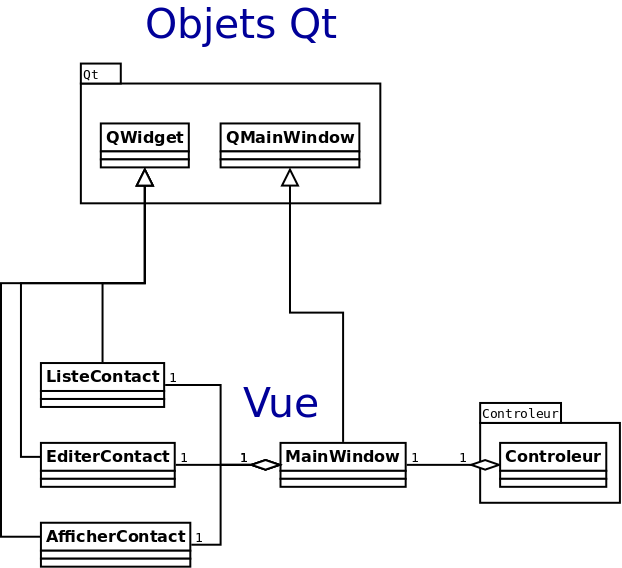
\includegraphics[scale=0.35]{../dia/ClassDiagramView.png}

La vue est composée d'une \texttt{MainWindow} et de six widgets \texttt{ListeContact}, \texttt{EditerContact}, \texttt{AfficherContact}, \texttt{LocEdit}, \texttt{StructureEdit} et \texttt{EnumEdit} qui servent à l'affichage et l'édition des champs et des contact dans la fenêtre.

On y trouve également les boîtes de dialogue \texttt{CritereTri}, \texttt{Rechercher} et \texttt{AjouterChamp} qui permettent à l'utilisateur d'entrée des informations lorsqu'il veut effectuer un tri, une recherche dans la liste des contacts ou ajouter un champ.

\chapter{Fonctionnalités implémentés}
\par
Voici la liste des fonctions implémentées:
\begin{itemize}
	\item Documentation du code dans son intégralité et utilisation de doxygen pour générer la doc
	\item Conception des classes permettant de représenter les contacts et les champs les décrivant.
	\item L'affichage de la liste des contacts
	\item L'ajout/suppression de contacts dans la liste
	\item L'affichage des détails d'un contact lors d'un clic sur celui-ci dans la liste
	\item La modification des champs d'un contact
	\item L'implémentation de tous les types de champ
	\item L'ajout/suppression de champs pour un contact
	\item La génération de champs par défaut lors de la création d'un contact
	\item La différentiation Personne/Organisme
	\item Le tri de la liste des contacts selon un critère
	\item La recherche dans la liste des contacts selon un critère
	\item L'import/export de la liste des contact en utilisant le format vCard
	\item L'import/export de la liste des contact en utilisant un format XML
	\item Deux langages sont gérés : Français et Anglais (automatiquement ajusté en fonction de la langue de la machine)
\end{itemize}

\section{Import/Export}

\subsection{vCard}
\par
Pour ce qui est du format vCard, toutes les classes du modèle possède une méthode \texttt{toVCard()} qui renvoie une \texttt{QString} correspondant à la conversion de ce champ en chaîne de caractère respectant le format vCard.

\subsection{XML}
\par
Quant au format XML, il exporte les champs et les contacts en utilisant \texttt{toString()}, du coup la méthode \texttt{toXML()} n'a besoin d'être implémentée que dans \texttt{Contact} et \texttt{Champ}.
\par
Syntaxiquement, le format XML se résume à une structure semblable à celle du modèle : une suite de \texttt{<Contact> ... </Contact>} avec des balise dont le nom est type du champ et qui possède un attribut \texttt{nomChamp} qui contient le nom de ce champ, et dont le contenu est la valeur du champ.




\chapter{Interface graphique}
\par
L'interface graphique contient une liste de contact à gauche et l'affichage ou bien l'édition des contacts à droite. On peut aussi sélectionner plusieurs boutons dans le menu afin d'afficher une fenêtre de recherche, de tri, d'ouverture de fichier, d'enregistrement de fichier.
\par
Chaque contact est précédé d'une image qui le représente (un logo ou une photo) si ce champ est renseigné.
\par
La vue des contacts est composé d'une liste de champ accompagné de leur valeur et pour certains champs d'icones renseignants sur les champs (par exemple le type de téléphone : fixe,mobile, ou bien le type d'adresse : home,work )
\par
En mode édition chaque champ est modifiable par un widget particulier : par exemple l'édition des dates peut se faire via l'affichage d'un calendrier, l'édition des adresses peut se faire ou bien via une ligne d'édition de texte ou bien via un tableau afin d'éditer chaque sous-champ séparé. Les autres type de champs sont eux aussi être édités par des widgets dédiés.
\par
Les photos peuvent être chargées à partir d'internet ou d'un fichier local.
\par
L'interface graphique se compose d'une barre de menu, d'une barre de raccourcis et d'un layout central.
\par
Toutes les fonctionnalités sont accessible via la barre de menu, et quasiment toutes le sont via la barre de raccourcis.
\par
Le layout central est divisé en trois layouts : la liste des contacts, l'affichage du contact et l'édition du contact.
Ces deux derniers ne sont jamais visibles simultanément.
\par
Options des menus :
Nouvelle liste (pour réinitialiser la liste de contact), Nouvelle personne, Nouvel organisme, Ouvrir, Enregistrer, Trier, Rechercher, Arrêter la recherche, Supprimer contact, Quitter.

\chapter{Conclusion}
\section{Résultats}
\par
Toutes les fonctionnalités demandées sont réalisés.
\par
Le modèle implémenté permet facilement d'intégrer d'autres types de champ en créant d'autres classes héritant de \texttt{Champ} ou d'une de ses filles/petites-filles.
\par

\section{Avancement personnel}
\par
Ce projet a permis d'apprendre mieux la partie modèle/vue de Qt.

Il nous a permis de mieux connaître la librairie Qt et qtcreator.


\end{document}